\renewcommand{\SourceFile}{1-parcours-de-tableaux/src/1-5.ml}

\section{Tri d'un petit nombre d'éléments}

Soit $n$ un entier $\geq 2$. Le but de cet exercice est d'étudier les algorithmes de tri d'un tableau de n éléments entiers, pour $n=3,4,5$ et 10. On ne compte que les comparaisons entre éléments du tableau, et on note $Comp(n)$ leur nombre.

\Q
Donner un algorithme, et écrire la fonction OCaml correspondante, pour trier un tableau de taille $n=3$ avec $Comp(n)=3$.\\
Même question avec $n=4$ et $Comp(n)=5$.\\
Même question avec $n=5$ et $Comp(n)=7$.

\Q
On suppose que $n=10$. On demande de préciser le nombre de comparaisons pour chacun des deux algorithmes basés sur les principes suivants (mais on ne demande aucune fonction OCaml dans cette question) :
\medskip

Algorithme 1. Faire deux listes de 5 éléments, utiliser deux fois l'algorithme précédent pour $n=5$ et fusionner les deux listes triées obtenues.
\medskip

Algorithme 2. Faire 5 paires d'éléments et trier les 5 plus grands de chaque paire à l'aide de l'algorithme pour $n=5$. Puis insérer les éléments restants dans la liste formée.

\Corrige
\vspace{.6cm}

Commençons par définir une fonction qui range dans l'ordre deux éléments d'un tableau \texttt{t} en positions \texttt{i} et \texttt{j} :

\lstinputlisting[linerange={1-6}]{\SourceFile}

\Q
Très facile avec 3 éléments : on met le plus petit élément en position 1 en le comparant aux deux autres, puis on classe les deux éléments restants :

\lstinputlisting[linerange={8-11}]{\SourceFile}

Pour 4 éléments : on classe les paires en position (0, 1) et (2, 3), puis on met les deux plus petits en position 0 et le plus grand des deux plus grands en position 3. Enfin, reste à classer les éléments en positions 1 et 2 :

\lstinputlisting[linerange={13-18}]{\SourceFile}

Une autre solution est de trier les 3 premiers éléments (3 comparaisons) puis d'insérer le quatrième, ce qui coûte 2 comparaisons supplémentaires en procédant par dichotomie, c'est-à-dire en commençant par l'élément du milieu.
\medskip

Avec 5 éléments : trier les 4 premiers éléments puis insérer le cinquième par dichotomie est ici trop coûteux : il faut 3 comparaisons pour insérer un élément dans une liste de taille 4. Cette solution nous coûterait $5+3=8$ comparaisons.
\medskip

Voici une solution en 7 comparaisons : on prend les 4 premiers éléments, on classe les paires (0, 1) et (2, 3) et on compare les deux plus grands éléments. La situation se résume à l'aide du diagramme (où $\texttt{a}\geq\texttt{b}\geq\texttt{c}$ et $\texttt{a}\geq\texttt{d}$) :

\begin{center}
    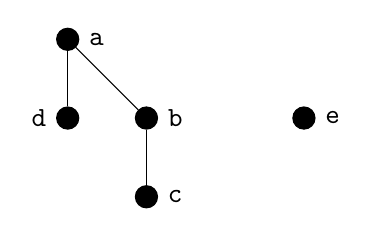
\begin{tikzpicture}[
        label distance=2pt,
        every node/.style={
            font=\ttfamily,
            draw,
            fill=black,
            circle,
            inner sep=0pt,
            minimum size=8pt}]
        \node[label=right:a] (A) at (1,2) {};
        \node[label=right:b] (B) at (2,1) {};
        \node[label=right:c] (C) at (2,0) {};
        \node[label=left:d] (D) at (1,1) {};
        \node[label=right:e] (E) at (4,1) {};

        \draw (A) -- (D);
        \draw (A) -- (B);
        \draw (B) -- (C);
    \end{tikzpicture}
\end{center}

On insère alors le cinquième élément $e$ dans la chaîne $a,b,c$ de longueur 3, ce qui coûte 2 comparaisons. Enfin, on insère le quatrième élément $d$ parmi les éléments inférieurs à $a$ dans l'ensemble $a,b,c,e$ ordonné, ce qui coûte deux comparaisons.
\medskip

On commence par définir une fonction utilitaire :

\lstinputlisting[firstline={20}]{\SourceFile}

La fonction est volumineuse mais ne pose pas de difficulté particulière.

\Q
Pour l'algorithme 1, le décompte est facile : on utilise deux fois la fonction \texttt{tri\_5}, ce qui conduit à 14 comparaisons. Reste à fusionner deux listes triées de 5 éléments. Or la fusion de deux listes triées de tailles respectives $m$ et $n$ requiert $m+n-1$ comparaisons, soit ici 9 comparaisons. On obtient un total de 23 comparaisons.
\medskip

Pour l'algorithme 2, après les 5 premières comparaisons et la fonction \texttt{tri\_5} appliquée aux 5 plus grands, on a la situation suivante :
\vspace{1.5cm}

\begin{center}
    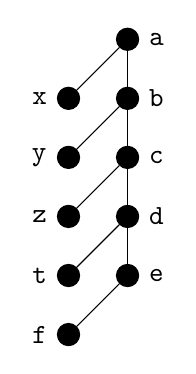
\begin{tikzpicture}[
        label distance=2pt,
        every node/.style={
            font=\ttfamily,
            draw,
            fill=black,
            circle,
            inner sep=0pt,
            minimum size=8pt}]
        \node[label=right:a] (A) at (.75,4.75) {};
        \node[label=right:b] (B) at (.75,4) {};
        \node[label=right:c] (C) at (.75,3.25) {};
        \node[label=right:d] (D) at (.75,2.5) {};
        \node[label=right:e] (E) at (.75,1.75) {};

        \node[label=left:x] (X) at (0,4) {};
        \node[label=left:y] (Y) at (0,3.25) {};
        \node[label=left:z] (Z) at (0,2.5) {};
        \node[label=left:t] (T) at (0,1.75) {};
        \node[label=left:f] (F) at (0,1) {};


        \draw (A) -- (B);
        \draw (B) -- (C);
        \draw (C) -- (D);
        \draw (D) -- (E);
        \draw (A) -- (X);
        \draw (B) -- (Y);
        \draw (C) -- (Z);
        \draw (D) -- (T);
        \draw (E) -- (F);

    \end{tikzpicture}
\end{center}

\newpage

Reste à insérer les 4 éléments $x$, $y$, $z$ et $t$ dans la chaîne ordonnée de longueur 6 $f,e,d,c,b,a$. On commence par insérer $z$ dans $d,e,f$ (2 comparaisons) puis on insère $t$ dans la liste qui comprend $f$, $e$ et éventuellement $z$ (encore deux comparaisons). On a :
\bigskip

\begin{center}
    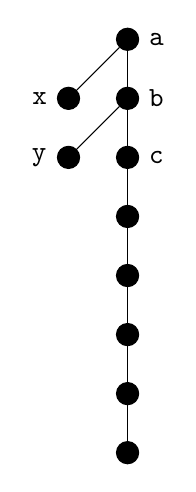
\begin{tikzpicture}[
        label distance=2pt,
        every node/.style={
            font=\ttfamily,
            draw,
            fill=black,
            circle,
            inner sep=0pt,
            minimum size=8pt}]
        \node[label=right:a] (A) at (.75,6.25) {};
        \node[label=right:b] (B) at (.75,5.5) {};
        \node[label=right:c] (C) at (.75,4.75) {};
        \node (S1) at (.75,4) {};
        \node (S2) at (.75,3.25) {};
        \node (S3) at (.75,2.5) {};
        \node (S4) at (.75,1.75) {};
        \node (S5) at (.75,1) {};

        \node[label=left:x] (X) at (0,5.5) {};
        \node[label=left:y] (Y) at (0,4.75) {};


        \draw (A) -- (B);
        \draw (B) -- (C);
        \draw (C) -- (S1);
        \draw (S1) -- (S2);
        \draw (S2) -- (S3);
        \draw (S3) -- (S4);
        \draw (S4) -- (S5);

        \draw (A) -- (X);
        \draw (B) -- (Y);

    \end{tikzpicture}
\end{center}
\bigskip

Insérer $x$ dans la chaîne de longueur 7 dont le plus grand élément est b requiert 3 comparaisons. Enfin, insérer $y$ dans une chaîne de longueur au plus 7 (longueur 6 si $x>b$, longueur 7 sinon) requiert également 3 comparaisons.
\medskip

Le nombre final de comparaisons est donc $5+7+2+2+3+3=22=Comp(10)$.
\medskip

Il se trouve que l'algorithme 2 est optimal. Bien sûr, c'est difficile à prouver ! D'une manière générale, la fonction $Comp\_min(n)$ qui donne le nombre minimal de comparaisons nécessaires pour trier $n$ éléments est très mal connue : on ne connaît pas d'expression exacte, juste un équivalent asymptotique en $O(n\log_2n)$.
\bigskip

\Fin
